\documentclass{article} % For LaTeX2e
\usepackage{graphicx}
\usepackage{subcaption}
\usepackage{amsmath}
\usepackage{nips13submit_e,times}
\usepackage{hyperref}
\usepackage{url}
\usepackage{booktabs, multicol, multirow, bigstrut, rotating} %for table import from excel
%\documentstyle[nips13submit_09,times,art10]{article} % For LaTeX 2.09

%Sets tiny font-size for tables
\let\oldtabular\tabular
\renewcommand{\tabular}{\scriptsize\oldtabular}

%%%%%%%%%%%%%%%%%%%%%%%%%%%%%%%%%%%%%%%%%%%%%%%%%%%%%%%%%%%%%%%%%%%%%%%
%MACROS: Using these to assign descriptive, permanent names to various values which might have their variable letter, etc. changed
% eg: \newcommand{\dataTrain}{X_train}
\newcommand{\bs}{\boldsymbol}

%VAR (vector autoregression) model macros
\newcommand{\VARnumVars}{N}
\newcommand{\VARnumTimesteps}{T}
\newcommand{\VARlag}{p}
\newcommand{\VARdata}{\bs{X}}
\newcommand{\VARmodel}{\bs{\Pi}}
\newcommand{\VARmodelrow}{\bs{\pi}}
\newcommand{\VARoffset}{\bs{c}}
\newcommand {\VARtrainData}{\VARdata_train}
\newcommand {\VARnoise}{\epsilon}
\newcommand{\predicted}{\hat}

\newcommand{\lassoMult}{\lambda^{(1)}}
\newcommand{\fusedLassoMult}{\lambda^{(2)}}

%%%%%%%%%%%%%%%%%%%%%%%%%%%%%%%%%%%%%%%%%%%%%%%%%%%%%%%%%%%%%%%%%%%%%%%


\title{Predicting Meteorological Values on a Spatial Grid}


\author{
Felipe Hern\'{a}ndez \\
University of Pittsburgh \\
\texttt{felher.c@gmail.com} \\
\And
Ben Humberston\\
Carnegie Mellon University \\
\texttt{bhumbers@cs.cmu.edu} \\
}

\newcommand{\fix}{\marginpar{FIX}}
\newcommand{\new}{\marginpar{NEW}}

\nipsfinalcopy

\begin{document}

\maketitle

%\begin{abstract}
%TODO
%\end{abstract}

\section{Introduction}
\label{sec:intro}

\subsection{Motivation}
\label{sec:motivation}
Weather forecasts are broadly used; from personal activity planning (What clothes should I wear today? Will it be a good time to plan outdoor events?); to large-scale economic decision-making (What activities should be prioritized on a crop next week? What precautions should the air-traffic controllers enforce on a given day?); to emergency preparation and response (What alternate routes should become available due to snow?, Where should the emergency vehicles be sent during a flood event?). The availability and accuracy of forecasts thus have a profound impact on human activities at many levels, both in measurable and unmeasurable aspects. However, predicting weather is a difficult research problem. Most often, physically-based models with global scale are used to forecast future conditions. In this project, we will instead take a machine learning approach focused on a local scale and attempt to predict atmospheric variables at specific geographic locations. The forecasts will be based on prior atmospheric system state in the neighborhood of a selected location. In particular, we will attempt to predict system variables such as pressure, precipitation, and temperature based on the previous values of these variables provided by regular historical satellite observations.

\subsection{Related Work}\label{sec:related_work}
Atmospheric sciences have always studied a variety of methods for weather forecasting. Many physical phenomena are involved in the state of the weather variables at a certain time, including energy and mass transfer between the sun, the different layers of the atmosphere, the ground, the oceans, etc. The development of physically-based forecasting models requires the incorporation of a wide variety of phenomena, such as used in \cite{Shuttleworth2012} and \cite{Harris2001}. The availability of meteorological measurements has helped the development of these methods, as well as other data-driven approaches. Machine Learning approaches have been used with isolated gauge data (\cite{Hong2008} and \cite{Paras2012}); more recently, it has also been applied to the data from emerging radar \cite{Ferraro1995} and satellite \cite{Yang2007} technologies.

One such satellite-based data product is the NLDAS (North American Land Data Assimilation System), a service hosted by the Goddard Earth Sciences Data and Information Services Center at NASA \cite{LDAS}. It provides hourly weather data for the US beginning in 1980. The data is provided on a regular grid with a resolution of 1/8\textsuperscript{th} of a degree in latitude-longitude coordinates. Table~\ref{fig:NLDAS_vars} shows the list of variables available from this data source. 

\begin{table}[htbp]
  \centering
    \begin{tabular}{l l l}
    \toprule
    \textbf{Name} & \textbf{Description} & \textbf{Units} \\
    \midrule
    precipitation & Accumulated height of precipitated water column & millimeters \\
    available potential energy & 180-0 mb above ground Convective Available Potential Energy & Joules per kilogram \\
    \% convective precipitation & Fraction of total precipitation that is convective & none \\
    LW radiation & Long wave radiation flux downwards (surface) & watts per square meter \\
    SW radiation & Short wave radiation flux downwards (surface) & watts per square meter \\
    potential evaporation & Potential evaporation & millimeters \\
    surface pressure & Surface pressure & pascals \\
    specific humidity & 2 m above ground Specific humidity & none \\
    temperature 2 m & 2 m above ground Temperature & kelvin \\
    zonal wind speed & 10 m above ground Zonal wind speed & meters per second \\
    meridional wind speed & 10 m above ground Meridional wind speed & meters per second \\
    \bottomrule
    \end{tabular}%
    \caption{Meteorological variables available from NLDAS-2}
  \label{fig:NLDAS_vars}%\
\end{table}%

\section{Method}
\label{sec:method}

\subsection{Linear Regression}
Linear regression was used as an initial na\"{\i}ve approach to estimate the values of the weather variables. For each cell in the NLDAS-2 map, we have a value $y$ to predict, and a set of variables $\bs{x}$ which are inputs into the prediction. We train a linear regression model of the form $y = \bs{w}^T\bs{x}$, where $y$ is a linear combination of the values in vector $\bs{x}$. The vector $\bs{w}$ contains the coefficients of the linear model.

If we take a time frame made of $T$ one-hour steps, and look at all the $n$ cells in the study area, we have $T*n$ examples of $y$ values as a function of the corresponding values of $\bs{x}$. These values can be arranged in a vector $\bs{y}$ of size $T*n$, and a matrix $\bs{X}$ of size $(T*n) \times f$, with $f$ being the number of features in the linear model. We can compute the coefficient vector $\bs{w}$ using the following equation:
\begin{equation}
	\bs{w} = (\bs{X}^T \bs{X})^{-1}\bs{X}^T\bs{y}
\end{equation}
Additionally, using the same formulation, a polynomial regression can be computed by adding higher degree terms into the set of features.


\subsection{VAR model}
The linear regression model is intended as a baseline solution. Our main work uses a vector autoregressive (VAR) model in order to simulate and predict the evolution of the meteorological system over time.  We adopt the formulation and estimation strategy given in \cite{SpluTimeSeries2006}.  The model describes the system values at time $t$ given some number of prior system states $p$, which is the lag order of the model:\
\begin{equation}
\VARdata_t = \VARoffset + \VARmodel_1 \VARdata_{t-1} + ... +  \VARmodel_\VARlag \VARdata_{t-\VARlag} + \VARnoise_t,
\end{equation}
Here, $\VARdata_i$ is the system state at the $i^{th}$ timestep; each of these is an $N$-length vector formed by reshaping and concatenating the various geographic grids of observed data variables (eg: temperatures, pressures, and so on at each of the grid points). Note that the data is offset to zero-mean over all time steps and normalized to have unit variance. $\VARoffset$ is a constant offset. Each $\VARmodel_j$ specifies the $N \times N$ model coefficient matrix which defines weighted sums of the observed data at timestep $t - j$. In a model of lag order $\VARlag$, the new state $\VARmodel_t$ is a sum of linear combinations of prior system states $\VARmodel_j \VARdata_{t-j}$ from timestep $t-1$ to $t - \VARlag$. Finally, $\VARnoise_t$ is a zero-mean noise generator which is uncorrelated between time steps which introduces innovations to the process.

This system can be solved for the unknown $\VARmodel_j$ matrices using ordinary least squares by rewriting it as a system of equations where each row is the equation for one system variable at one time step:
\begin{equation}
	\bs{x}_i = \bs{Z} \VARmodelrow_i+ \bs{e}_i,  i=1,...,\VARnumVars
\end{equation}
Given that we are training on $T$ timesteps, $\bs{x}_i$ is a $T$-length vector giving the values for the $i^{th}$ system variable over all timesteps (eg: ``atmospheric pressure at ($20^\circ$ N, $34^\circ$ W) over a 24 hour period''). $\bs{Z}$ is a $T \times k$ matrix ($k = np + 1$), where the $t^{th}$ row is defined as $\bs{Z}_t = (1, \VARdata_{t-1}^T, \VARdata_{t-2}^T,...,\VARdata_{t-p}^T$), $\bs{e}_i$ is a zero-mean noise vector, and $\VARmodelrow_i$ is a $k$-length vector of coefficients to be determined. Using a typical least squares approach, we create an estimate $\predicted{\VARmodelrow}_i$ for $i = 1,...,\VARnumVars$, yielding our estimation for the full model:
\begin{equation}
	\predicted{\VARmodel} \in (k \times N) 	=  \begin{bmatrix} \predicted{c} \\ \predicted{\VARmodel}_i^T \\ \vdots \\ \predicted{\VARmodel}_\VARlag^T \end{bmatrix} 
					=  \begin{bmatrix} \predicted{\VARmodelrow}_1 & \hdots & \predicted{\VARmodelrow}_\VARnumVars \end{bmatrix}
	\label{eq:model_matrix}
\end{equation}

\subsection{Lasso}
Our data set includes a number of metereological variable types which are defined on the geographic grid. Since we suspect that not every data observation will be critical to modeling the system's evolution, we intend to use the lasso regularization \cite{Tibshirani1996} to enforce sparse feature selection. This changes our least squares problem slightly. We now wish to minimize the quantity 
\begin{equation}
	\sum\limits_{i=1}^\VARnumVars (\bs{x}_i - \bs{Z} \VARmodelrow_i)^2  + \lassoMult \sum\limits_{i=1}^k \sum\limits_{j=1}^\VARnumVars | \VARmodel_{i,j} |
\end{equation}
$\lassoMult$ is the Lagrange multiplier on the lasso constraints. This is a convex optimization and should be solvable using standard tools.

\subsection{Fused Lasso}
Additionally, we have reason to believe that the model coefficients $\VARmodel$ should exhibit some temporal consistency so that the relationship of parameters within ranges of timesteps $\VARmodel_{t1} ... \VARmodel_{t2}$ show constant trends. To explore this, we turn to the fused lasso, a modified version of lasso introduced by \cite{Tibshirani2005}. It is useful for time series data because it encodes the relationship between successive parameters. Our modified objective function for fused lasso is 
\begin{equation}
	\sum\limits_{i=1}^\VARnumVars (x_i - Z \VARmodelrow_i)^2  
	+ \lassoMult \sum\limits_{j=1}^k \sum\limits_{i=1}^\VARnumVars | \VARmodel_{i,j} |  
	+ \fusedLassoMult  \sum \limits_{i=1}^\VARnumVars \sum \limits_{t=2}^T | \VARmodelrow_{i,t} - \VARmodelrow_{i,t-1} |
\end{equation}
Here, $\fusedLassoMult$ is the Lagrange multiplier on the additional constraints for fused lasso. Refer to Equation~\ref{eq:model_matrix} for the relationship between $\VARmodelrow$ terms and $\VARmodel$.

The fused lasso regularization may be particularly useful if we examine the VAR model behavior over longer time scales than hour-by-hour weather. There are, naturally, seasonal variations in meteorological variables, and it is possible that the system behavior encoded by the model coefficients $\VARmodel$ is also dynamic based on the time of year.

\subsection{Evaluation}
The success of our model depends on its ability to correctly forecast (predict) the new system state at time $t$ based on the system state at times $t-\VARlag$ to $t-1$. Since there is some inherent noise $\VARnoise$ in the variables of the system, the primary goal is to minimize the residual of predicted system state $\predicted{\VARdata}_t$ relative to the actual historical observation $\VARdata_t$ to within some reasonable range of this noise term.  The size of our data set allows us to easily train on a subset of the full data and test on another independent set (eg: train on data from the year 2004, test on data from the year 2007).

We intend to use cross-validation in order to ensure that our data does not overfit to any particular data set. Additionally the lag order $\VARlag$ of the VAR model provides a way of controlling the model complexity; larger values of $\VARlag$ yield more complex models. We can observe the training and test error for models trained for different lags and thus estimate an optimal lag size which is large enough to capture the system dynamics but small enough to avoid overfitting.

\section{Results}
\label{sec:results}
Currently, we have implemented both a simple linear regression model as well as a standard VAR($\VARlag$) model which predicts new system values given prior system states.

\subsection{Linear Regression}
A small region around Pittsburgh was selected as the test case for this method. It spans a 6 x 6 grid of 10 km x 10 km size cells. Hourly records for each cell were used from 9/15/2010 to 10/15/2010.

Four linear regression models were computed for each one of the meteorological values in NLDAS-2. The first two were determined assuming a static framework: computing the current value if all the other current values are known. The first regression only used terms of degree one, while the second used terms of degree two (the quadratic term of each value plus the all the product terms between any two values). The third and fourth models were also of degree one and two, but were developed to estimate the values of the weather variables in the next time step (an hour into the future) given the current values of all the variables in the current time step.

In order to test the performance of each model, five runs were executed randomly taking 10\% of the examples as a testing set, and then computing the root mean square error (RMSE) of the predictions for both the training and the testing set. Table~\ref{fig:lin_reg_testing_error} shows the relative errors of the trained models on the test set for each variable, as the ratio between the RMSE and the standard deviation of the entire sample of each variable.

\begin{table}[htbp]
  \centering
    \begin{tabular}{ccccc}
    \toprule
    \multirow{2}[2]{*}{\textbf{Variable}} & \multicolumn{2}{c}{\textbf{Current time step}} & \multicolumn{2}{c}{\textbf{Next time step}} \\
          & \textbf{degree 1} & \textbf{degree 2} & \textbf{degree 1} & \textbf{degree 2} \\
    \midrule
    precipitation & 101.28\% & 91.45\% & 87.33\% & 84.21\% \\
    potential energy & 79.15\% & 76.41\% & 22.20\% & 18.83\% \\
    \% convective & 89.82\% & 84.78\% & 72.68\% & 73.00\% \\
    LW radiation & 61.11\% & 59.93\% & 28.88\% & 29.39\% \\
    SW radiation & 41.81\% & 42.32\% & 25.01\% & 24.60\% \\
    potential evaporation & 32.58\% & 30.65\% & 29.34\% & 27.29\% \\
    surface pressure & 93.67\% & 88.34\% & 8.60\% & 8.52\% \\
    specific humidity & 47.63\% & 44.35\% & 38.11\% & 35.48\% \\
    temperature & 46.22\% & 46.34\% & 12.61\% & 11.82\% \\
    wind speed & 77.16\% & 78.18\% & 21.14\% & 19.90\% \\
    \textbf{Average} & \textbf{67.04\%} & \textbf{64.27\%} & \textbf{34.59\%} & \textbf{33.30\%} \\
    \bottomrule
    \end{tabular}%
  \caption{Relative testing errors of the linear regression models}
  \label{fig:lin_reg_testing_error}%
\end{table}% 

As can be seen, the high relative errors for most cases indicate that the proposed approach is still not adequate for forecasting. However, there is a strong indication that variables are highly dependent on their previous values (since the estimation for the next time step is mostly better), and that there is a small improvement when higher order terms are included into the model. Additionally, there is a wide variation in the quality of the prediction between variables. There is also virtually no difference between training and testing errors, so we can conclude that the models are not over-fitted.

\subsection{VAR Model}
We illustrate an example of the output from the VAR model in Figure~\ref{fig:var_data_example}. Thus far, this model has also shown poor performance, where the errors in the model output are very large relative to the expected noise in each observed variable.

\begin{figure}[t]
\centering
\begin{subfigure}[b]{0.4\textwidth}
	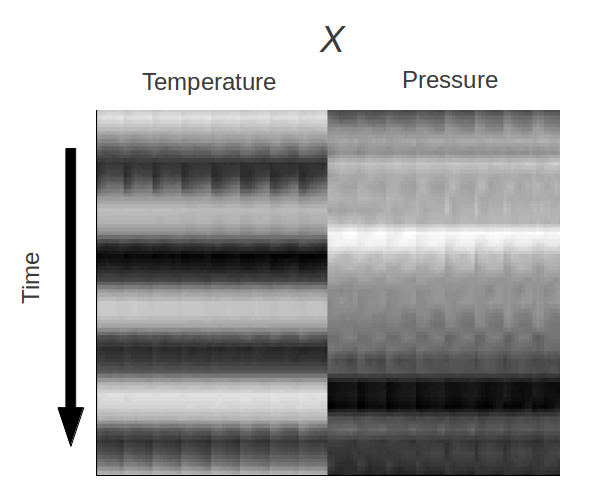
\includegraphics[width=1.0\textwidth]{./var_data_example.png}
	\caption{Input data comprised of temperature and pressure values on a small grid region}
\end{subfigure}
\hspace{0.05\textwidth}
\begin{subfigure}[b]{0.2\textwidth}
	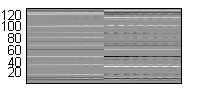
\includegraphics[width=1.0\textwidth]{./var_params_lag_1.png}
	\caption{Trained model coefficients assuming a lag order $\VARlag = 1$}
\end{subfigure}
\hspace{0.05\textwidth}
\begin{subfigure}[b]{0.2\textwidth}
	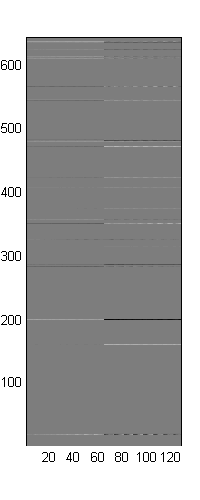
\includegraphics[width=1.0\textwidth]{./var_params_lag_5.png}
	\caption{Trained model coefficients assuming a lag order $\VARlag = 5$}
\end{subfigure}
\caption{An illustrative example of the input data $\VARdata$ and trained output model $\predicted{\VARmodel}$ obtained using different lag parameters. The data is comprised of hourly samples over a 4-day window. Each row in $\VARdata$ corresponds to all the observed values at a particular timestep, where the 2D gridded values for each variable type (in this case, surface temperature and pressure) are reshaped into row vectors. Note that the large, monochrome gray regions in each $\predicted{\VARmodel}$ indicates significant sparsity of the model, which was not expected until after we apply lasso regularization. }
\label{fig:var_data_example}
\end{figure}

There are several possible reasons for this which we intend to investigate. First, the VAR model assumes a \emph{stationary} process, and our current preprocessing of the data before fitting the model may not guarantee this assumption. Additionally, not all variables which may affect predictions are yet included in this model (eg: wind speeds, elevation, etc.). We will observe whether adding these terms improves predictive accuracy before testing the (fused) lasso-regularized version of this model.

\section{Appendix}

\subsection{Updated Timeline}
\begin{itemize}
\item Training and performance evaluation of VAR model – Week 1 (Nov. 18-24)
\item Training and performance evaluation of fused lasso VAR regression – Week 1 (Nov. 18-24)
\item Comparison of linear regression, static VAR approach, and fused lasso regression – Week 2 (Nov. 25 – Dec. 1)
\item Poster preparation – Week 2 (Nov. 25 – Dec. 1)
\item Report preparation – Week 3 (Dec. 2-8)
\end{itemize}


\bibliographystyle{plain}
\bibliography{10_701_Project_Refs}

\end{document}